\section{Part IV: The Formalized, Falsified Predictor}\label{sec:part4}

Parts I and III found opposite results in two domains. The obvious candidate law says the difference is quantitative: the supervision gap grows with the witness fiber, Definition~\ref{def:fiber}'s count, formalized in Lean. Part~IV formalized that law, pre-registered it, and refuted it.

\subsection{The registered design}

Six conditions, each a system of eight operations on a 28-bit state with witness length $L = 6$. Vocabulary, witness length, state representation, output length, and operation names are identical across conditions; names are opaque (\texttt{OP0}\dots\texttt{OP7}) so no structure leaks through labels. Only the algebra differs, interpolating between the two end cases proved in Section~\ref{sec:formal}. I computed fiber sizes \emph{exactly}, by full enumeration of all $8^6 = 262{,}144$ witnesses per condition: readable 1.0, free 1.0, q25 2.8, q50 29.7, q75 349.1, abelian 2581.0. Four arms per condition (trace / pair / endpoint / shuffle) at matched character budget, trained under the Part~III protocol (Pythia-160M, fp32, stage-1 lr $5\times10^{-5}$, stage-2 lr $2\times10^{-5}$, seed 0 registered, seeds 1 and 2 as replicates): 24 training runs in total. The eval asks the model to generate the witness from the endpoint pair; the primary metric is token accuracy over the six operation slots, chance $= 0.125$. The witness alphabet is disjoint from the state alphabet, so copying the input cannot beat chance and no echo correction is required. Registered predictions: P4a, the gap grows with $\log_2$ fiber (slope $>0$, $p<0.05$, $r^2 \geq 0.5$); P4b, \texttt{free} exceeds \texttt{readable} by $\geq 0.05$ (same fiber, opposite invertibility); P4c, the sanity anchor: on \texttt{readable}, where the end state literally contains the witness, all arms exceed 0.80 and the gap is below 0.05; P4d, content share above 50\% in the high-fiber conditions.

\subsection{The failed sanity check}

P4c failed on the first condition. Every arm scored at chance, 0.121 to 0.161 against a chance level of 0.125, because the state was rendered as a binary string and the model could not decode nibbles. The registration said that if the sanity anchor fails, no other prediction in the file may be interpreted. I stopped the sweep after one condition, on the registered rule.

\subsection{The computation that retired the design}

Working through the failure exposed something deeper than the encoding. The gap must vanish at \emph{both} ends of the fiber axis. At fiber 1 with an easy encoding, the inverse is learnable and stage~2 alone teaches both arms, so the low end fails. At large fiber, the witness is not determined by the endpoints, so \emph{no} arm can exceed a near-chance ceiling, and the high end fails. Table~\ref{tab:ceiling} makes this exact: Bayes ceilings by full enumeration, and the maximum possible gap (ceiling minus chance) at each condition.

\begin{table}[htbp]
\centering\footnotesize
\caption{Exact Bayes ceilings (generation-from-endpoints eval, $L = 6$). The maximum gap any supervision format could produce collapses at both ends of the fiber axis. \emph{Source: project data~\cite{appliedrepo2026}.}}
\label{tab:ceiling}
\begin{tabular}{lccc}
\toprule
condition & mean fiber & Bayes ceiling & max gap \\
\midrule
readable & 1.0 & 1.000 & 0.875 \\
free & 1.0 & 1.000 & 0.875 \\
q25 & 2.8 & 0.915 & 0.790 \\
q50 & 29.7 & 0.739 & 0.614 \\
q75 & 349.1 & 0.514 & 0.389 \\
abelian & 2581.0 & 0.190 & 0.065 \\
\bottomrule
\end{tabular}
\end{table}

At the abelian end the maximum achievable gap is 0.065, within noise of any realistic measurement. And at fiber 1, the \texttt{free} condition caps \emph{both} arms computationally: the witness there is determined by the endpoints only through inverting six mixing maps, which the model cannot do either. The low end fails too, which also invalidated P4b as registered.

\begin{figure}[htbp]
\centering
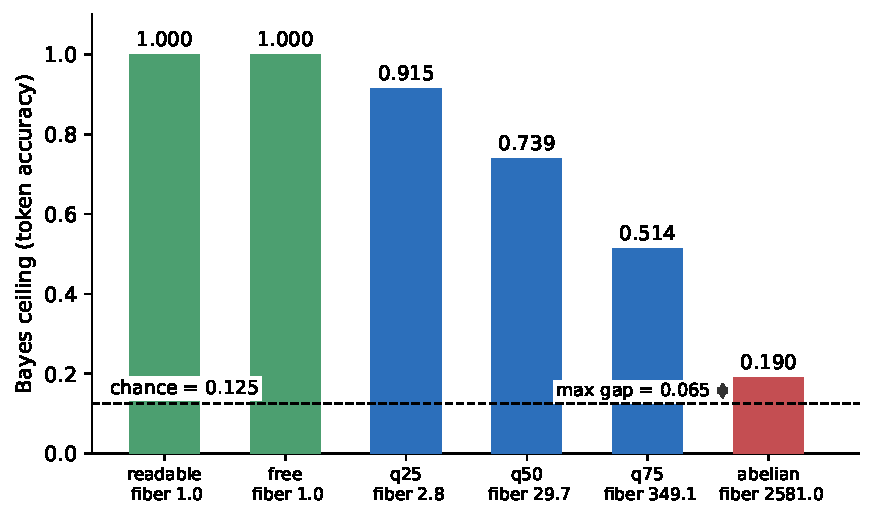
\includegraphics[width=0.85\textwidth]{figs/f5_ceilings.pdf}
\caption{The impossibility figure. Exact Bayes ceilings per condition (fiber sizes in parentheses), chance level dashed. No monotone law from fiber size to the supervision gap can pass through these bars. \emph{Source: figure created by the author from project data~\cite{appliedrepo2026}.}}
\label{fig:ceiling}
\end{figure}

The registration had also planned, as illustration, to place Parts I and III on the fitted curve after the fact. With the curve retired, the Part~I versus Part~III contrast stands as a recoverability-controlled domain difference, measured by the $0.003$ diagnostic, not as evidence for a quantitative law.

\subsection{The claim, exactly sized}

{\sloppy
For this family of operation systems, under generation-from-endpoints evaluation, \emph{no monotone law from fiber size to the supervision gap can exist}: the achievable gap is bounded by ceilings that collapse at both ends of the axis. This is a claim about this family and this evaluation mode, not a general impossibility theorem. Its provenance is the point: the quantity was defined in Lean, its consequences computed exactly in \texttt{ceiling.py}, and the conjecture it refutes was pre-registered before the computation refuted it. The standalone lesson is the pair of \texttt{readable} and \texttt{free}: identical fiber (1.0), opposite computational invertibility. Information and computation are separate axes, and the formal quantity, fiber size alone, is incomplete by construction.
\par}

\subsection{A second falsified predictor}\label{sec:secondneg}

The fiber law died of its own ceilings. A sharper candidate arrived from conversation: Sebastien Seboih conjectured a cost-function version. Attach a linear cost with nonzero coefficients on every state component, aggregated along the witness. Then endpoint data (start, end, total cost) should fail to recover the cost function where paths are ambiguous, while traces succeed. This is the right kind of conjecture: it names a quantity, a mechanism, and a predicted gap.

The test is exact linear algebra (\texttt{identifiability.py}, all $8^6$ paths per system). For each condition, build what the endpoint pair tells the regression (fiber-averaged state components and total cost) and what the trace adds, and compute the rank each side gives cost recovery (Table~\ref{tab:ident}).

\begin{table}[htbp]
\centering\footnotesize
\caption{Cost-function identifiability, exact computation over all $8^6$ paths per system. Rank of the cost-recovery regression from trace features and from endpoint (pair) features; deficit is the dimension the endpoint features cannot see. \emph{Source: project data~\cite{appliedrepo2026}.}}
\label{tab:ident}
\begin{tabular}{lcccc}
\toprule
opset & $\log_2$ fiber & rank trace & rank pair & deficit \\
\midrule
readable & 0.00 & 19 & 19 & 9 \\
free & 0.00 & 28 & 28 & 0 \\
q25 & 1.51 & 28 & 28 & 0 \\
q50 & 4.89 & 28 & 28 & 0 \\
q75 & 8.45 & 28 & 28 & 0 \\
abelian & 11.33 & 9 & 9 & 19 \\
\bottomrule
\end{tabular}
\end{table}

Two readings settle it. Wherever the dynamics are rich, the fiber-mean features span the full 28-dimensional space, so an exact endpoint learner recovers the cost completely (deficit 0). Where the deficit is nonzero (readable, abelian), it binds the trace arm identically: unexcited components are unidentifiable from any data, the persistence-of-excitation condition hiding inside the conjecture's ``nonzero coefficients'' clause. The relative trace-versus-pair deficit is zero in every system. The conjectured gap cannot occur here, and the design was stopped before registration.

One quantity survives: the finite-sample noise of the endpoint learner is the within-fiber cost variance, which here is strictly monotone in $\log$ fiber (0.0004, 0.1395, 0.2792, 0.3978, 0.5534 for free, q25, q50, q75, abelian). That suggests a variance-alone sample-complexity predictor. Direct simulation of an OLS endpoint learner falsifies it: samples to excess risk 0.05 give $n/\mathrm{variance}$ ratios of 789, 663, 654, 199 across q25, q50, q75, abelian, non-constant and direction-inverted. The highest-variance system was the easiest, because its endpoint features span only 9 of 28 dimensions.

The two-factor quantity, variance times effective rank of the endpoint features, repairs the predictor: $n\,\epsilon/(\mathrm{variance}\times\mathrm{rank})$ = 1.41, 1.18, 1.17, 1.10 across the same systems, constant within a factor of 1.3 where variance alone spans $4.0\times$ and flips sign. Sizing: for linear learners this is textbook regression theory confirmed on these systems; whether neural learners obey it is open, and Section~\ref{sec:limitations} names it as a registered open question.

The structural point: three candidate predictors entered this project through this route (the fiber, cost-function identifiability, variance-alone sample complexity), and exact computation killed all three before a single wasted training run (artifacts: \texttt{REGISTERED\_NEGATIVE.md} with its dated addenda, \texttt{identifiability.py}, \texttt{variance.py}, and \texttt{ols\_sample\_complexity.py}). A fourth survived the exact-computation filter and had to be taken to an experiment; it is Part~VI (Section~\ref{sec:part6}).

\section{Part V: The Mechanism, Tested by Budget}\label{sec:part5}

\subsection{Question and design}

Part~IV retired the information-theoretic explanation. Two mechanism candidates remain for the Part~III advantage. \emph{Data efficiency}: the pair arm never sees witness tokens in stage~1, so it must learn the witness vocabulary and distribution from stage~2 alone; enough stage-2 data should erase the difference. \emph{Structural transfer}: stage-1 trace exposure conveys something about the state-to-tactic correspondence that endpoint data cannot supply at any stage-2 budget. The registered design holds stage~1 fixed per arm and varies the stage-2 budget over $N \in \{125, 250, 500, 1000, 2000, 4000\}$, with nested draws (each smaller set a prefix of the next), so that at a given $(N, \text{seed})$ every arm sees identical examples in identical order. Registered predictions: P5a, the gap decreases with $\log_2 N$ (slope $< 0$, $p < 0.05$); P5b, at $N = 4000$ the gap is below $+0.02$ and no longer significant; P5c, the anchor: at $N = 2000$ the gap lands within $\pm 0.025$ of Part~III's $+0.054$.

Two known slack sources were stated before running, so the anchor check is distributional, not exact: Part~III drew its stage-2 set with \texttt{random.sample} while this design uses shuffle-then-prefix to keep budgets nested, and stage~1 runs as a separate process, so the random state entering stage~2 differs. A small-$N$ caveat was also stated: at $N = 125$ stage~2 is roughly four optimizer steps; all six points enter the regression regardless.

\subsection{Results}

\begin{table}[htbp]
\centering\small
\caption{Part V budget curve, seed 0. The pair arm plateaus from $N=1000$; the trace arm keeps improving to its best at $N=4000$. \emph{Source: project data~\cite{appliedrepo2026}.}}
\label{tab:budget}
\begin{tabular}{rcccc}
\toprule
$N$ & \texttt{pw\_trace} & \texttt{pw\_pair} & gap & $p$ \\
\midrule
125 & $-0.0736$ & $-0.1823$ & $+0.1086$ & $2.0\times10^{-27}$ \\
250 & $-0.0699$ & $-0.1483$ & $+0.0784$ & $3.0\times10^{-15}$ \\
500 & $-0.0715$ & $-0.1397$ & $+0.0682$ & $3.5\times10^{-11}$ \\
1000 & $-0.0573$ & $-0.1302$ & $+0.0729$ & $3.1\times10^{-14}$ \\
2000 & $-0.0718$ & $-0.1245$ & $+0.0527$ & $5.8\times10^{-9}$ \\
4000 & $-0.0427$ & $-0.1256$ & $+0.0829$ & $1.2\times10^{-13}$ \\
\bottomrule
\end{tabular}
\end{table}

\begin{figure}[htbp]
\centering
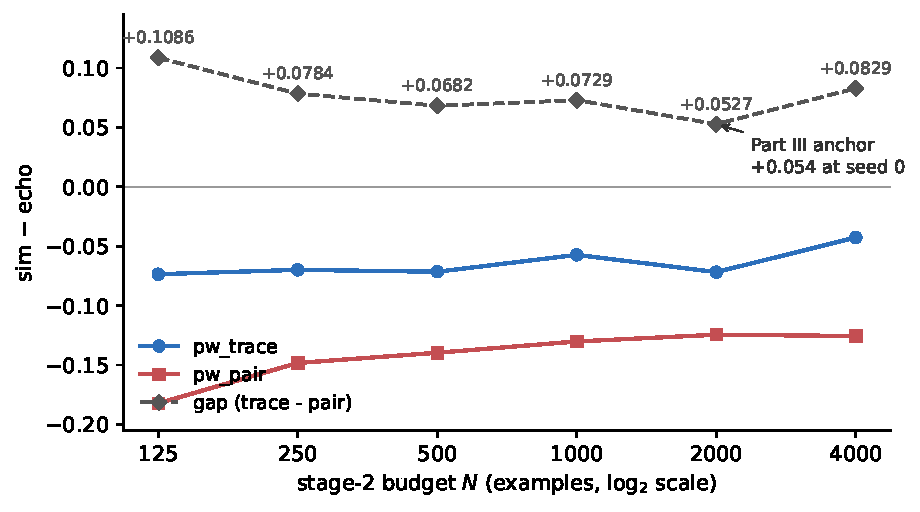
\includegraphics[width=0.9\textwidth]{figs/f4_budget_curve.pdf}
\caption{The budget curve: arm scores and the gap against the stage-2 budget on a $\log_2$ scale. The gap at $N=2000$ anchors Part~III; the gap at $N=4000$ is the largest since $N=125$. \emph{Source: figure created by the author from project data~\cite{appliedrepo2026}.}}
\label{fig:budget}
\end{figure}

Verdicts. P5c \textbf{passed}: $+0.0527$ against the $+0.054$ anchor, a miss of 0.0013. The pipeline measures what Part~III measured. P5a \textbf{failed}: slope $-0.0057$ on six points, $r^2 = 0.335$, $p = 0.229$, no significant decay. P5b \textbf{failed decisively}: at $N = 4000$ the gap is $+0.0829$, $p = 1.2\times10^{-13}$, the largest since the four-optimizer-step regime at $N = 125$. Extrapolating the flat, insignificant slope anyway gives a zero-crossing near $2^{22.9} \approx 8.0$ million examples; I report it as an extrapolation beyond the tested range, which is what it is. The pattern shows in the arm scores, not just the gap: the pair arm plateaus at $\approx -0.125$ from $N = 1000$ onward, while the trace arm keeps improving to its best score at $N = 4000$. The 4000-vs-2000 uptick ($+0.030$, $p = 0.079$) is suggestive only, and I label it as such.

\subsection{The registered conditional: decomposition at \texorpdfstring{$N = 4000$}{N = 4000}}

Because P5b failed, the pre-registered conditional took effect: train \texttt{pw\_shuffle} stage~1, fine-tune once at $N = 4000$, and decompose the surviving gap. Content (trace $-$ shuffle): $+0.0563$ (176 to 99, $p = 5.2\times10^{-6}$). Format (shuffle $-$ pair): $+0.0266$ (175 to 108, $p = 9.0\times10^{-5}$). Content share 68\%, against Part~III's 73\% at $N = 2000$ (76\% across seeds). The composition of the gain survives the budget test, not only its size.

\begin{figure}[htbp]
\centering
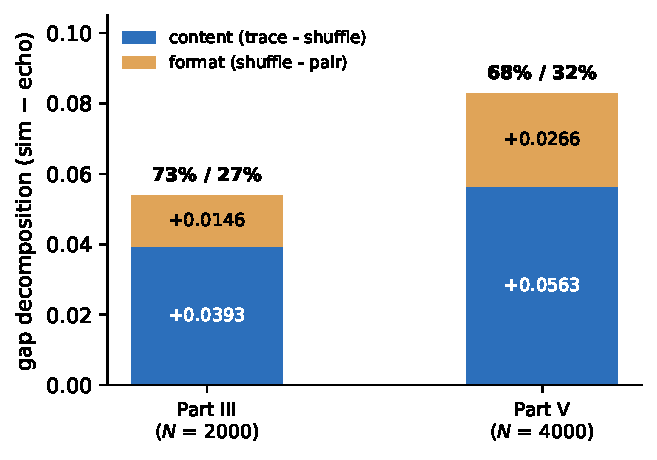
\includegraphics[width=0.47\textwidth]{figs/f6_decomposition.pdf}
\caption{Content/format decomposition at the two operating points. The content share is stable (73\% to 68\%) across a doubling of the stage-2 budget. \emph{Source: figure created by the author from project data~\cite{appliedrepo2026}.}}
\label{fig:decomp}
\end{figure}

\subsection{The final claim, exactly sized}

The trace advantage in this domain is majority witness content, is not format familiarity, and is not purchasable with endpoint fine-tuning data across a $32\times$ budget range. Two uncertainty statements belong inside the claim, not in a footnote: the curve is single-seed, and Part~III's own cross-seed magnitude swing is a factor of two. The honest statement is that the gap persists everywhere it was measured, with magnitude known only to that factor.
